\documentclass[conference]{IEEEtran}
\usepackage{cite}
\usepackage{amsmath,amssymb,amsfonts}
\usepackage{algorithmic}
\usepackage{graphicx}
\usepackage{textcomp}
\usepackage{xcolor}
\def\BibTeX{{\rm B\kern-.05em{\sc i\kern-.025em b}\kern-.08em
    T\kern-.1667em\lower.7ex\hbox{E}\kern-.125emX}}
\begin{document}

\title{Project: COVID-19 Assisted Diagnosis\\


\author{\IEEEauthorblockN{Frie Van Bauwel\textsuperscript{1}}
\and
\IEEEauthorblockN{Lotte Van de Vreken\textsuperscript{2}}
\and
\IEEEauthorblockN{Marcin Jedrych\textsuperscript{3}}
\and
\IEEEauthorblockN{Xueting Li\textsuperscript{4}}

\and


\textsuperscript{1,2,3,4}  Master of Science in statistical data analysis - computational statistics\hfill}}

\maketitle



\section{Introduction}
Within this project on medical image classification, two deep learning models are trained to classify X-ray images of lungs as COVID-positive or COVID-negative images. Further, the Grad-CAM visualization technique is used to be able to show on which areas of an X-ray image are mainly used by the algorithm to decide whether an image shows a person affected with COVID or a person not affected with COVID. This report describes first how the data are explored, preprocessed and augmented (section \ref{sec:task_1}). It then explains how a baseline model, using a convolutional network, was fitted (section \ref{sec:task_2}) and how transfer learning was used to make use of the pre-trained ResNetV2 model (section \ref{sec:task_3}). Section \ref{sec:task_4} describes in which the Grad-CAM visualisation is used to understand why missclassifications happen in the best performing model trained in the previous tasks.
After the conclusion (section \ref{sec:conclusion}), the report describes how this project was divided between all group members (section \ref{sec:author_contributions}). The final section entails our use of generative AI during the project (section \ref{sec:generative_AI}).


\section{Task 1: Data Exploration, Pre-Processing and Augmentation}\label{sec:task_1}

As a first step, a data exploration was carried out. The dataset consists out of 1600 training images, 400 validation images and 200 test images. The amount of training images can be considered as quite limited, hence a risk of overfitting exists. Other potential challenges for automatic classification that become clear with having a first look at the images are the subtle differences in COVID versus normal chest X-rays, as well as the variability in brightness, contrast, and the exact part of the lungs shown on the X-ray between pictures. Both challenges are addressed by using normalization and augmentation techniques as described below. Based on the pixel statistics and label distribution, the datasets appear to be fairly uniformly divided.  The mean values and standard deviations of the pixel values are comparable across the sets: training (mean = 0.53, std = 0.25), validation (mean = 0.55, std = 0.25), and test (mean = 0.56, std = 0.26). This finding indicates that the image intensity is consistent. The class distribution in all three sets also looks well balanced. There are no consistent differences in image quality between the COVID and normal X-ray images. However, it can be observed that some pictures have a much higher intensity distribution than others, creating the need for proper normalization. In some pictures, artefacts like wires could be seen, which can lead to lower model performance. To reduce the training time and memory usage, the pictures were downsampled from 299x299 to 128x128 resolution. This allows for faster runtimes without losing too much information. Additionally, it makes the picture more general thus reducing the risk that the model will overfit on small artefacts in the pictures. The images were normalized using dataset statistics: the mean and standard deviation of all pixels in the training, validation and test dataset were used as normalization statistic. The X-ray images contain black-and-white images thus all three image channels contain the same information and could be normalized using the same statistic. To augment the data, pictures were slightly shifted in width, rotated with a maximum range of 15 degrees and zoomed with a maximum factor of 0.2. These augmentation patterns were chosen because they represent still realistic X-ray variations, as patients can be positioned slightly more on the side, can be a bit closer or further from the imager or can be slightly tilted. Other augmentations such as vertical or horizontal flip would create unrealistic images that would never occur in real-life examples.


%Includes tables with quantitative results (Table~\ref{table:example}) and images (Fig.~\ref{fig:example}) from your project while carefully explaining their meaning and how you produced them.
%\begin{table}[htbp]
%\caption{Table Type Styles}
%\begin{center}
%\begin{tabular}{|c|c|c|c|}
%\hline
%\textbf{Table}&\multicolumn{3}{|c|}{\textbf{Table Column Head}} \\
%\cline{2-4} 
%\textbf{Head} & \textbf{\textit{Table column subhead}}& \textbf{\textit{Subhead}}& \textbf{\textit{Subhead}} \\
%\hline
%copy& More table copy$^{\mathrm{a}}$& &  \\
%\hline
%\multicolumn{4}{l}{$^{\mathrm{a}}$Sample of a Table footnote.}
%\end{tabular}
%\label{table:example}
%\end{center}
%\end{table}


\section{Task 2: Building the baseline model}\label{sec:task_2}

\begin{figure}[h] \centering 						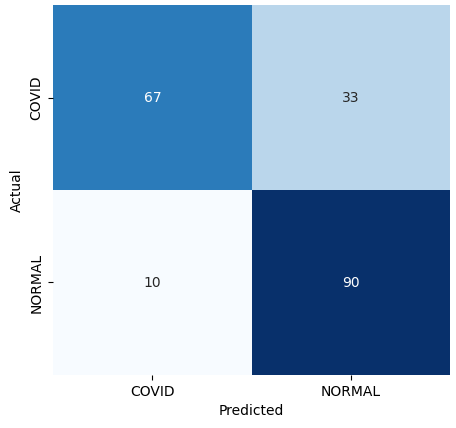
\includegraphics[width=0.9\columnwidth]{fig_task2_confusionmatrix.png} 
	\caption{Confusion matrix of the test data classified by the final baseline model.} 
	\label{fig:task2_confusionmatrix} 
\end{figure}


\begin{figure*}[h] \centering 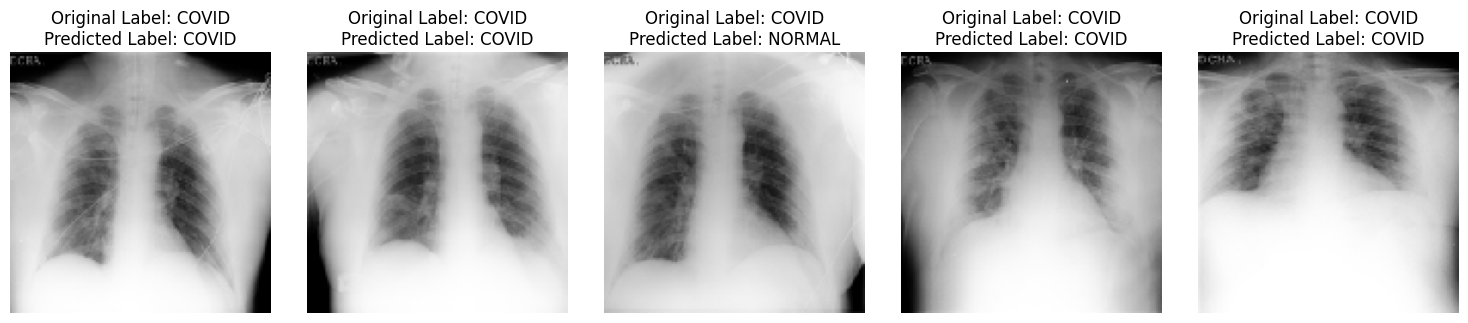
\includegraphics[width=0.9\textwidth]{fig_task2_examples_images_label_vs_predictedlabel.png} 
	\caption{Sample of test images with the real and predicted label, as classified by the final baseline model.} 
	\label{fig:task2_image_examples} 
\end{figure*}


\begin{figure*}[h] \centering 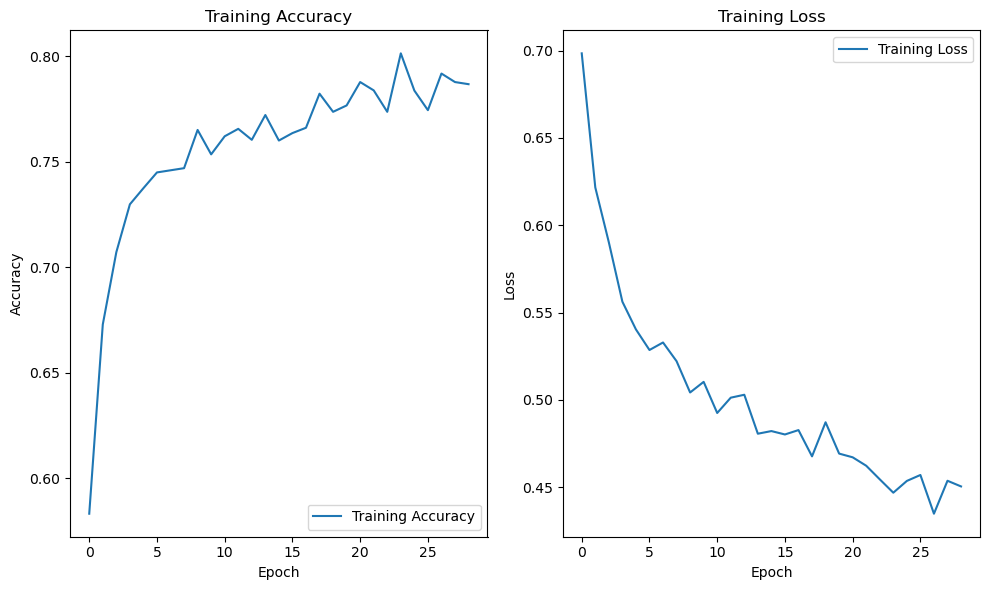
\includegraphics[width=0.6\textwidth]{fig_task2_training_curves_train_final_model.png}
	\caption{The training curves of the loss and accuracy of the final baseline model where the model was trained based on the combination of validation and training data.} 	
	\label{fig:task2_curves_final} 
\end{figure*}

\begin{figure*}[h] \centering 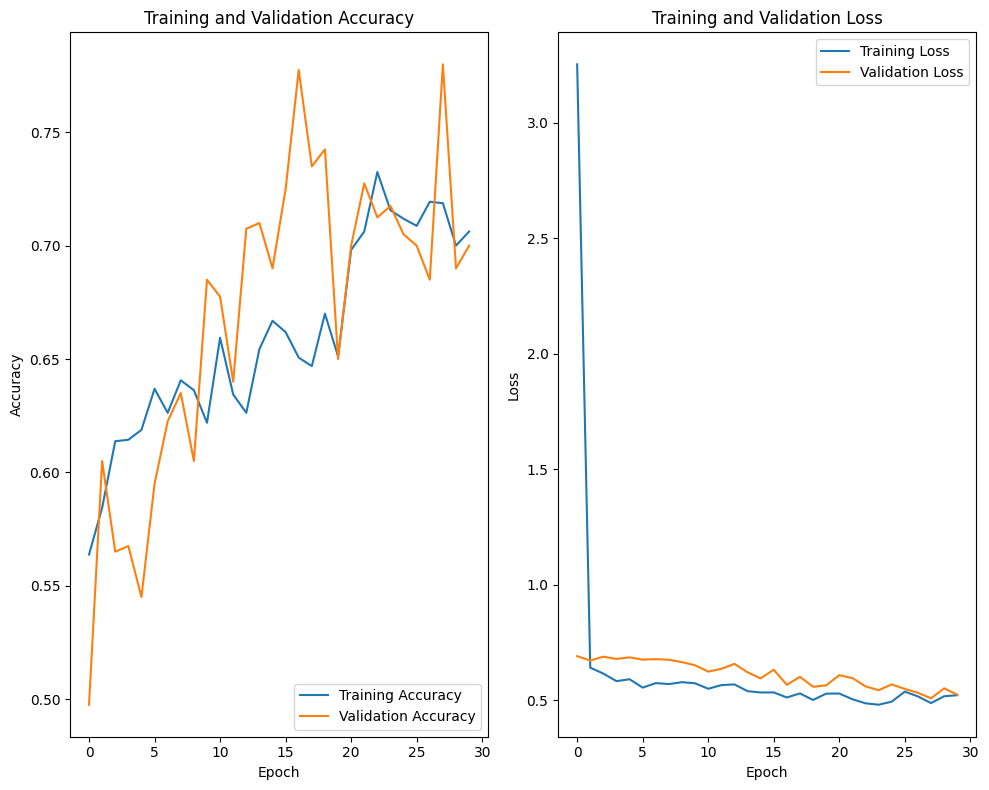
\includegraphics[width=0.6\textwidth]{fig_task2_training_curves_train_validation_initial_model.png} 
	\caption{The training and validation curves of the loss and accuracy of the initial baseline model before the hyperparameter tuning.} 
	\label{fig:task2_curves_initial} 
\end{figure*}

\section{Task 3: Transfer Learning}\label{sec:task_3}


Within task 3, a neural network is built using the transfer learning approach. In other words, a pretrained model is used as a basis to built a model, hereby making it possible to use a network with many layers even though a limited set of training data is available. 
In this case, the ResNet50V2, a model consisting of 50 layers, is used as the pretrained model. After the ResNet50V2 model, four extra layers are added. First, a GlobalAveragePooling2D layer is added to reduce the spatial dimensions. Then, a 128-node dense layer with relu-activation is added in combination with a dropout layer to reduce risk of overfitting. A final single-node dense layer with sigmoid activation was used to get the binary output.

After setting the model architecture, the hyperparameters of the added layers are tuned using a general grid search. The tuned parameters consist of the  batch size, learning, and dropout rates. Table XXXXX shows the XXranges/combinations that are used during the hypertuning process and indicated the optimal outcomes for each hyperparameter. 
While tuning the hyperparameters, the pretrained parameters in the ResNet50V2-layers remain unchanged. Early stopping based on the validation loss is used with a patience of five steps. After this tuning step, a model is trained during XX epochs based on the training and validation data. 
Another, final, model is trained in which the ResNet50V2-layers are unfrozen, hence fine-tuning the weights in these layers is possible. The training curves of the model before unfreezing the ResNet50V2-layers is visualized in figure \ref{fig:task3_curves_final_hyperparams}, the training curves of the model after unfreezing is visualized in figure \ref{fig:task3_curves_final_resnet}.

The training curves of both trained models within this task look smooth and have shape coming close to the ideal training curve. 
The model where the ResNet50V2 model parameters are finetuned shows a higher accuracy and lower loss (respectively X and X in the fully trained model) than the model without the extra finetuning (respectively X and X in the fully trained version).
This hints towards better performance of the finetuned model, but might also indicate a bigger chance of overfitting on the training dataset (consisting of the provided training and validation set). As requested in the task, no training of this model was done using the validation set as holdout-samples, hence this is hard to judge.
Comparing these curves to the training curve in task 2, XXXX

As a final step in this task, the finetuned model is evaluated using the test set. Both the confusion matrix (\ref{fig:task3_confusionmatrix}) and the calculated accuracy of XX shows a major improvement compared to the baseline model. 
This increase in performance is probably due to the transfer learning approach which caused a smoother learning curve that converged faster to decent results with only a limited increase in learning time, even with limited training data. 
However, still XX out of XX samples are misclassified as COVID and XX samples are misclassified as normal.
This indicates a big difference in performance compared to the training data, which implies overfitting. Even though the added layers on top of the pretrained ResNet50V2 are meant to restrict this problem. 
One way to alleviate this overfitting is to introduce bigger transformations in the training set, or add more training data if possible. Alternatively, starting with a lower resolution can also help.
Another way to improve the results is using a pretrained model specifically trained on medical images such as CheXNet instead of ResNet50V2 as a basis of the transfer learning.

\begin{figure}[h] \centering 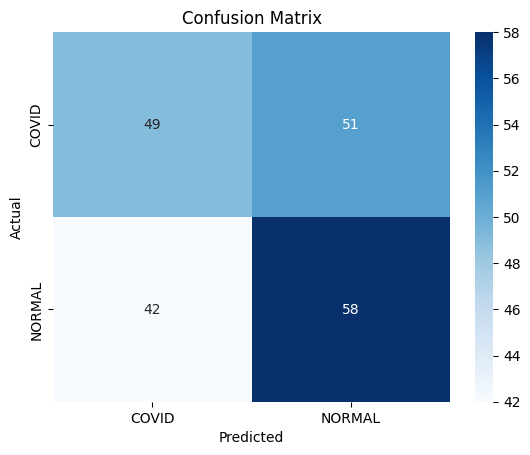
\includegraphics[width=0.9\columnwidth]{fig_task3_confusionmatrix.png} \caption{Confusion matrix of the test data classified by the final transfer model (with tuned hyperparameters and fine-tuned weights of the ResNet50v2 model).} \label{fig:task3_confusionmatrix} 
\end{figure}


\begin{figure*}[h] \centering 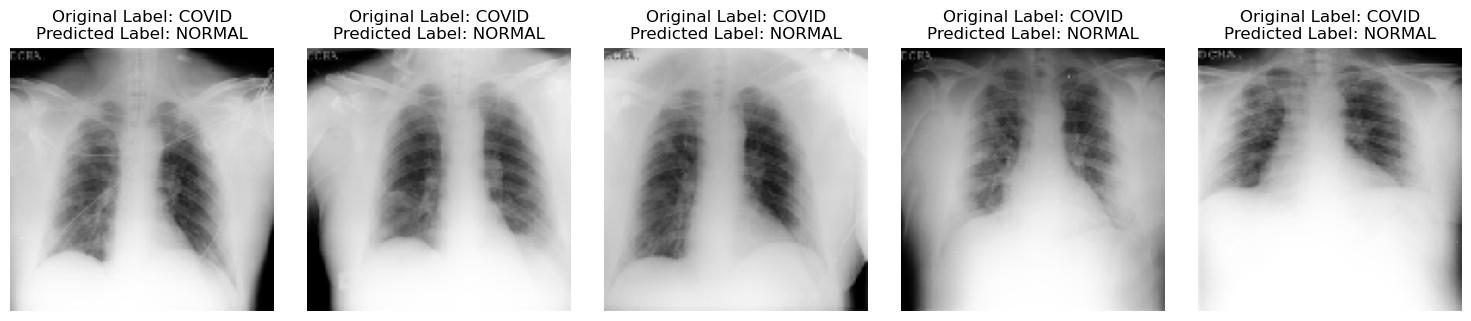
\includegraphics[width=0.9\textwidth]{fig_task3_examples_images_label_vs_predictedlabel.png} 
	\caption{Sample of test images with the real and predicted label, as classified by the final transfer model.} 
	\label{fig:task3_image_examples} 
\end{figure*}


\begin{figure*}[h] \centering 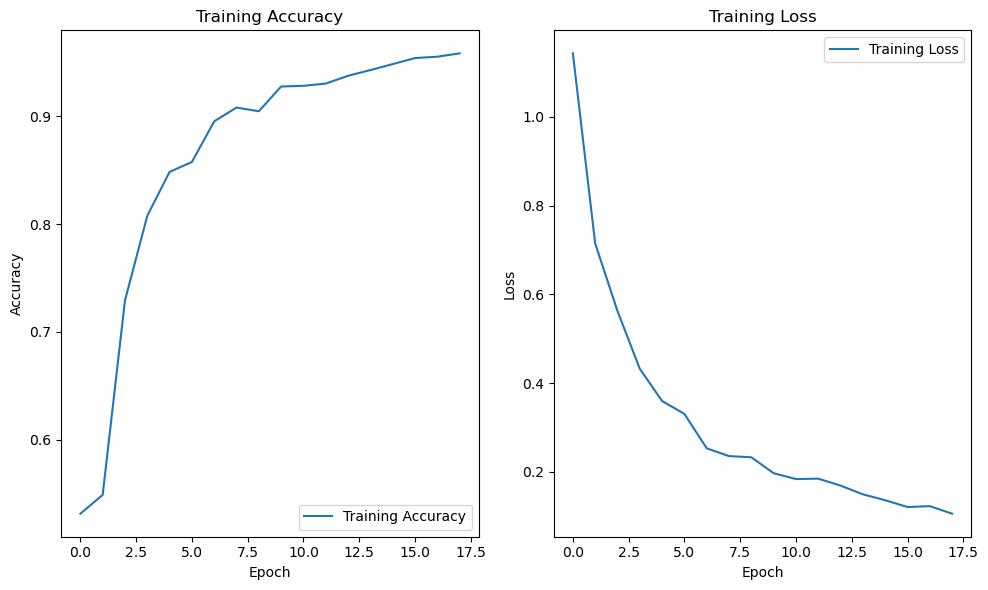
\includegraphics[width=0.6\textwidth]{fig_task3_training_curves_train_model_finetuned_resnet.png} 
	\caption{The training curves of the loss and accuracy of the final transfer model with tuned hyperparameters and weights of the ResNet50v2 where the model was trained based on the combination of validation and training data.} 
	\label{fig:task3_curves_final_resnet} 
\end{figure*}

\begin{figure*}[h] \centering 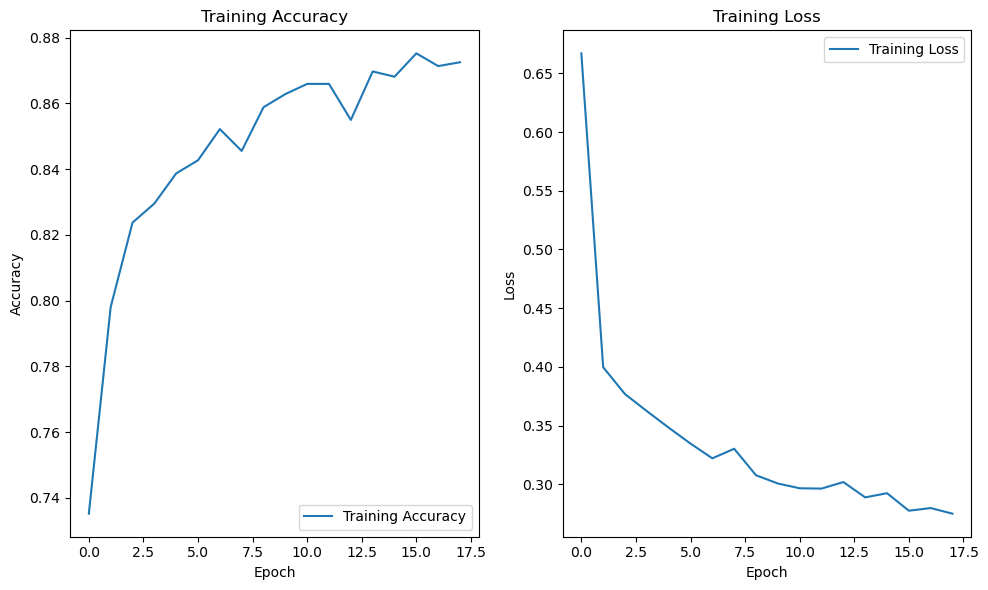
\includegraphics[width=0.6\textwidth]{fig_task3_training_curves_train_model_tuned_hyperparameters.png} 
	\caption{The training curves of the loss and accuracy of the final transfer model with tuned hyperparameters, but the original weights of the ResNet50v2, where the model was trained based on the combination of validation and training data.} 
	\label{fig:task3_curves_final_hyperparams} 
\end{figure*}

\begin{figure*}[h] \centering 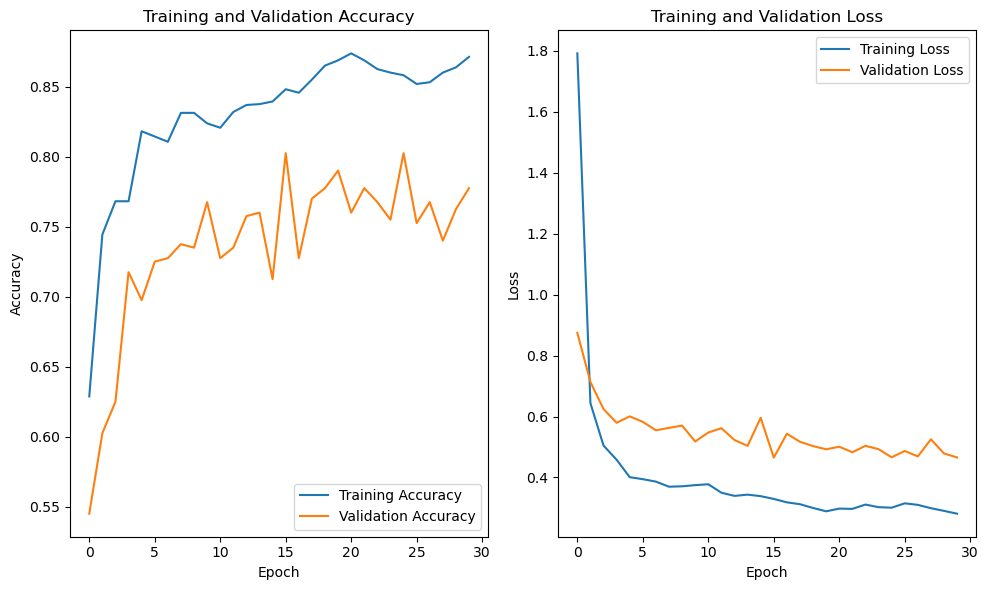
\includegraphics[width=0.6\textwidth]{fig_task3_training_curves_train_validation_initial_model.png} 
	\caption{The training and validation curves of the loss and accuracy of the initial transfer model.} \label{fig:task3_curves_initial} 
\end{figure*}

\section{Task 4: Explainability through Grad-CAM}\label{sec:task_4}

Grad-CAM (Gradient-weighted Class Activation Mapping), introduced by Selvaraju et al. in 2017, is a technique developed to provide visual insight into the decision-making process of convolutional neural networks (CNNs) \cite{b8}. CNNs are powerful models for image classification, but they are often criticized for their "black box" nature—producing accurate predictions without a clear explanation of how those predictions were formed. Grad-CAM addresses this issue by generating heatmaps that highlight the most relevant regions of an input image with respect to a specific class prediction. These heatmaps are constructed using the gradients of the target class scores with respect to the activations in the final convolutional layers, effectively showing which parts of the image influenced the model’s decision.
This interpretability is particularly important in domains such as medical imaging or autonomous driving, where understanding why a model made a decision is just as critical as the decision itself. gradient-based techniques have since become a widely used approach in explainable AI (XAI) \cite{b9}. 
For our project, we followed the Keras tutorial \cite{b10} that used a CNN with multiple output classes. We initially adjusted our model to do the same for two classes (COVID and Normal). However, we later found we could change the algorithm to make it work with a single scalar logit as output, representing the confidence for one class (e.g., COVID). We found that Grad-CAM could be applied by interpreting the scalar logit as the evidence for one class and its negative as the evidence for the other class (since the sigmoid output ensures that the total probability across both classes sums to one). This insight allowed us to use Grad-CAM effectively for a scalar-output binary classification model. Having two class labels (COVID and Normal) or only one scalar output does not affect predictions or interpretability of the Grad-CAM explanations. Whether the model produces two logits or a single scalar, the highlighted regions will be the same, as the underlying decision process remains equivalent.
Our Grad-CAM visualizations revealed that the model focuses particularly on the lung regions, which are medically relevant. It appears to detect opacities or structural anomalies consistent with COVID-19. However, the technique also helped us uncover potential model biases. In some cases, the Grad-CAM showed focus on irrelevant features such as cables or background artifacts, suggesting the model may have learned spurious correlations from the training data. 
Moreover, Grad-CAM proved useful in understanding misclassifications. In several incorrect predictions, we observed that the model was influenced by visual noise such as unusual patient posture. If this would have appeared more frequently in the opposite class, the model may have learned to associate these irrelevant features with that class, leading to incorrect predictions. 
Based on these insights, if we were to collect more data and retrain the model, we would prioritize minimizing visual biases by standardizing patient positioning, removing non-diagnostic artifacts (e.g., cables), and ensuring a balanced dataset across age and other demographic factors. These steps would help the model focus more effectively on clinically meaningful features, improving both accuracy and trustworthiness.

\begin{figure}[h] \centering 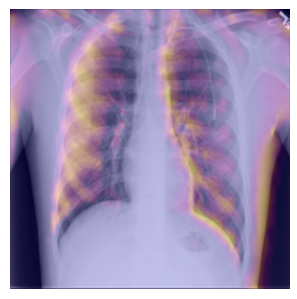
\includegraphics[width=0.8\columnwidth]{gradcam_example.png} \caption{Example Grad-CAM heatmap highlighting lung regions associated with a COVID-positive classification.} \label{fig:gradcam_example} \end{figure}

\section{Conclusions}\label{sec:conclusion}

\section{Author contributions and collaboration}\label{sec:author_contributions}
In first instance, the tasks were divided as follows:
\begin{itemize}
	\item Task 1: Marcin Jedrych and Frie Van Bauwel, 
	\item Task 2: Marcin Jedrych and Xueting Li,
	\item Task 3: Lotte Van de Vreken and Frie Van Bauwel,
	\item Task 4: Marcin Jedrych and Lotte Van de Vreken.
\end{itemize}

According to this division, everyone made sure there was a first version of the code for their assigned task. Afterwards, questions and unclarities in each task were discussed, after which everyone checked and complemented the first draft of the code of each task. Task 4 was kept until the other tasks were almost done. For the text, first an answer to the questions was formulated by the assigned people to each task, after which everyone Read them and complemented where the need was felt. Some questions were discussed at length before an answer was formulated.

\section{Use of Generative AI}\label{sec:generative_AI}
Generative AI was used to fix bugs in the code for all tasks except task 1. It was also used to get a first version of some parts of the code to plot the images for all tasks except task 1. Suggested code was however always looked at critically and never taken over one-on-one.

\subsection{Figures and Tables}
\paragraph{Positioning Figures and Tables}




\section*{References}
Example References:
\begin{thebibliography}{00}
\bibitem{b1} G. Eason, B. Noble, and I. N. Sneddon, ``On certain integrals of Lipschitz-Hankel type involving products of Bessel functions,'' Phil. Trans. Roy. Soc. London, vol. A247, pp. 529--551, April 1955.
\bibitem{b2} J. Clerk Maxwell, A Treatise on Electricity and Magnetism, 3rd ed., vol. 2. Oxford: Clarendon, 1892, pp.68--73.
\bibitem{b3} I. S. Jacobs and C. P. Bean, ``Fine particles, thin films and exchange anisotropy,'' in Magnetism, vol. III, G. T. Rado and H. Suhl, Eds. New York: Academic, 1963, pp. 271--350.
\bibitem{b4} K. Elissa, ``Title of paper if known,'' unpublished.
\bibitem{b5} R. Nicole, ``Title of paper with only first word capitalized,'' J. Name Stand. Abbrev., in press.
\bibitem{b6} Y. Yorozu, M. Hirano, K. Oka, and Y. Tagawa, ``Electron spectroscopy studies on magneto-optical media and plastic substrate interface,'' IEEE Transl. J. Magn. Japan, vol. 2, pp. 740--741, August 1987 [Digests 9th Annual Conf. Magnetics Japan, p. 301, 1982].
\bibitem{b7} M. Young, The Technical Writer's Handbook. Mill Valley, CA: University Science, 1989.
\bibitem{b8} R. R. Selvaraju, M. Cogswell, A. Das, R. Vedantam, D. Parikh, and D. Batra, ``Grad-CAM: Visual Explanations from Deep Networks via Gradient-Based Localization,'' in Proc. IEEE Int. Conf. Comput. Vis. (ICCV), 2017, pp. 618--626.
\bibitem{b9} M. Mersha, K. Lam, J. Wood, A. K. AlShami, and J. Kalita, ``Explainable artificial intelligence: A survey of needs, techniques, applications, and future direction,'' *Neurocomputing*, vol. 599, p. 128111, Sep. 2024.
\bibitem{b10} Keras Team, ``Grad-CAM class activation visualization,'' *Keras Documentation*, https://keras.io/examples/vision/grad_cam/, accessed May 7, 2025.

\end{thebibliography}
\end{document}
